\section{Batterien (Akkus)}

\textbf{Elektrochemische Speicher}
\begin{itemize}
    \item Zusammenschaltung mehrerer elektrochemischer Zellen
    \item Jede elektrochemische Zelle besteht aus zwei räumlich getrennten Elektroden, 
          die über einen Elektrolyten als ionenleitende Phase miteinander verbunden sind
    \item An den Elektroden findet eine in zwei Halbreaktionen getrennte Redoxreaktion statt
    \item Energie als im äußeren Stromkreis fließende Elektronen
\end{itemize}

\textbf{Einteilung}
\begin{itemize}
    \item Primär- oder Sekundärzellen
    \item Niedertemperatur-Batterien (z.B. Blei-, Nickel- und Lithium-Batterien)
    \item Hochtemperatur-Batterien (z.B. Natrium-Batterien)
    \item Interner oder externer Speicher (z.B. Redox-Flow-Batterien)
\end{itemize}

\subsection{Nennkapazität $C_{\text{nenn}}$}

\begin{minipage}[t]{0.23\columnwidth}
$
\boxed{C_{\text{nenn}} = \frac{C_{\text{nutzbar}}}{\mathrm{DOD_{Zul}}}}
$
\end{minipage}
\hfill
\begin{minipage}[t]{0.73\columnwidth}
    \renewcommand{\arraystretch}{1.2}
        \begin{tabular}{@{} l p{4.5cm} l @{}}
            $[C_{\text{nenn}}]$     & Nennkapazität der Batterie \dotfill          & $\mathrm{kWh}$ \\
            $[C_{\text{nutzbar}}]$  & Nutzbare Kapazität \dotfill                  & $\mathrm{kWh}$ \\
            $[\mathrm{DOD_{Zul}}]$          & Zulässige Entladetiefe \dotfill   & $-$ \\
\end{tabular}
\end{minipage}



\subsection{Vollzyklen $N_{\text{voll}}$}

\begin{minipage}[t]{0.25\columnwidth}
$
\boxed{N_{\text{voll}} = N_{\text{teil}} \cdot \mathrm{DOD_{Entl}}}
$
\end{minipage}
\hfill
\begin{minipage}[t]{0.71\columnwidth}
    \renewcommand{\arraystretch}{1.2}
        \begin{tabular}{@{} l p{4.5cm} l @{}}
            $[N_{\text{voll}}]$  & Anzahl geleisteter Vollzyklen \dotfill          & $-$ \\
            $[N_{\text{teil}}]$  & Anzahl Teilzyklen \dotfill                        & $-$ \\
            $[\mathrm{DOD_{Entl}}]$       & Entladetiefe (entnommen) \dotfill & $-$ \\
    \end{tabular}
\end{minipage}


\subsection{Gesundheitszustand der Batterie (SOH)}

\begin{minipage}[t]{0.32\columnwidth}
$
\boxed{\text{SOH} = 1 - \frac{N_{\text{voll}}}{N_{\text{zykl}}}\cdot (1 - \text{EOL})}
$
\end{minipage}
\hfill
\begin{minipage}[c]{0.58\columnwidth}
    Definition EOL bei 80 \% der Nennkapazität $C_{\mathrm{nenn}}$ (EN 60896) (normalerweise EOL = 0.8)
\end{minipage}

\vspace{0.1cm}

\begin{minipage}[t]{0.48\columnwidth}
    \renewcommand{\arraystretch}{1.2}
    \begin{tabular}{@{} l p{2.8cm} l @{}}
        $[\text{SOH}]$        & State of Health     \dotfill    & $\mathrm{\%}$ \\
        $[N_{\text{voll}}]$   & Geleistete Vollzyklen               \dotfill              & $-$ \\
    \end{tabular}
\end{minipage}
\hfill
\vrule width 1pt
\hfill
\begin{minipage}[t]{0.48\columnwidth}
    \renewcommand{\arraystretch}{1.2}
    \begin{tabular}{@{} l p{2.8cm} l @{}}
        $[N_{\text{zykl}}]$   & Zyklenfestigkeit                    \dotfill                   & $-$ \\
        $[\text{EOL}]$        & End-of-Life                  \dotfill & $-$ \\
    \end{tabular}
\end{minipage}



\subsection{Ladezustand (SOC)}

\begin{minipage}[t]{0.23\columnwidth}
$
\boxed{\text{SOC} = \frac{\sum P_i \cdot t_i}{C_{\text{nutzbar}}}}
$
\end{minipage}
\hfill
\begin{minipage}[t]{0.73\columnwidth}
    \renewcommand{\arraystretch}{1.2}
\begin{tabular}{@{} l p{4.5cm} l @{}}
    $[\text{SOC}]$         & Ladezustand der  Batterie \dotfill           & $\mathrm{\%}$ \\
    $[P_i]$                & Ladeleistung $i$ \dotfill      & $\mathrm{kW}$ \\
    $[t_i]$                 & Ladedauer Intervall $i$ \dotfill       & $\mathrm{h}$ \\
    $[C_{\text{nutzbar}}]$    & Nutzbare Kapazität \dotfill                 & $\mathrm{kWh}$ \\
\end{tabular}
\end{minipage}



\subsection{C-Rate}

\begin{minipage}[t]{0.23\columnwidth}
$
\boxed{C\text{-Rate} = \frac{P_{\text{Lade}}}{C_{\text{nenn}}}}
$
\end{minipage}
\hfill
\begin{minipage}[t]{0.73\columnwidth}
    \renewcommand{\arraystretch}{1.2}
\begin{tabular}{@{} l p{4.5cm} l @{}}
    $[C\text{-Rate}]$      & Verhältnis Ladeleistung zu Kapazität \dotfill & $\mathrm{1/h}$ \\
    $[P_{\text{Lade}}]$    & Ladeleistung \dotfill                         & $\mathrm{kW}$ \\
    $[C_{\text{nenn}}]$    & Nennkapazität der Batterie \dotfill           & $\mathrm{kWh}$ \\
\end{tabular}
\end{minipage}



\subsection{Lithium-Ionen-Batterien}

\subsubsection{Aufbau}

\begin{enumerate}
  \item Stromableiter
  \begin{itemize}
    \item Aluminium an der positiven Elektrode
    \item Kupfer an der negativen Elektrode
  \end{itemize}
  
  \item Positive Elektrode (Kathode, z.\,B. LiCoO\textsubscript{2})
  \begin{itemize}
    \item Metallische Struktur mit \glqq variablem\grqq{} Anteil an Li\textsuperscript{+}-Ionen
  \end{itemize}
  
  \item Negative Elektrode (Anode, z.\,B. Graphit/C\textsubscript{6})
  
  \item Separator (PP oder PE)
  \begin{itemize}
    \item Mikro-poröser Kunststoff, ionendurchlässig
  \end{itemize}
  
  \item Elektrolyt (z.\,B. LiPF\textsubscript{6})
  \begin{itemize}
    \item Ionenleiter (elektrisch nicht leitend)
  \end{itemize}
\end{enumerate}



\subsubsection{Aktivmaterialien}

\begin{minipage}[t]{0.6\columnwidth}
\textbf{Positive Elektrode:}
  \begin{itemize}
    \item Lithiumeisenphosphat (LFP)
    \item Lithium-Nickel-Mangan-Kobaltoxid (NMC)
    \item Lithiumkobaltoxid (LCO)
    \item Lithiummanganoxid (LMO)
    \item Lithium-Nickel-Kobalt-Aluminiumoxid (NCA)
  \end{itemize}
\end{minipage}
\hfill
\begin{minipage}[t]{0.36\columnwidth}
\textbf{Negative Elektrode:}
  \begin{itemize}
    \item Graphit (C\textsubscript{6})
    \item Lithiumtitanat (LTO)
  \end{itemize}
\end{minipage}



\subsubsection{Bauformen}

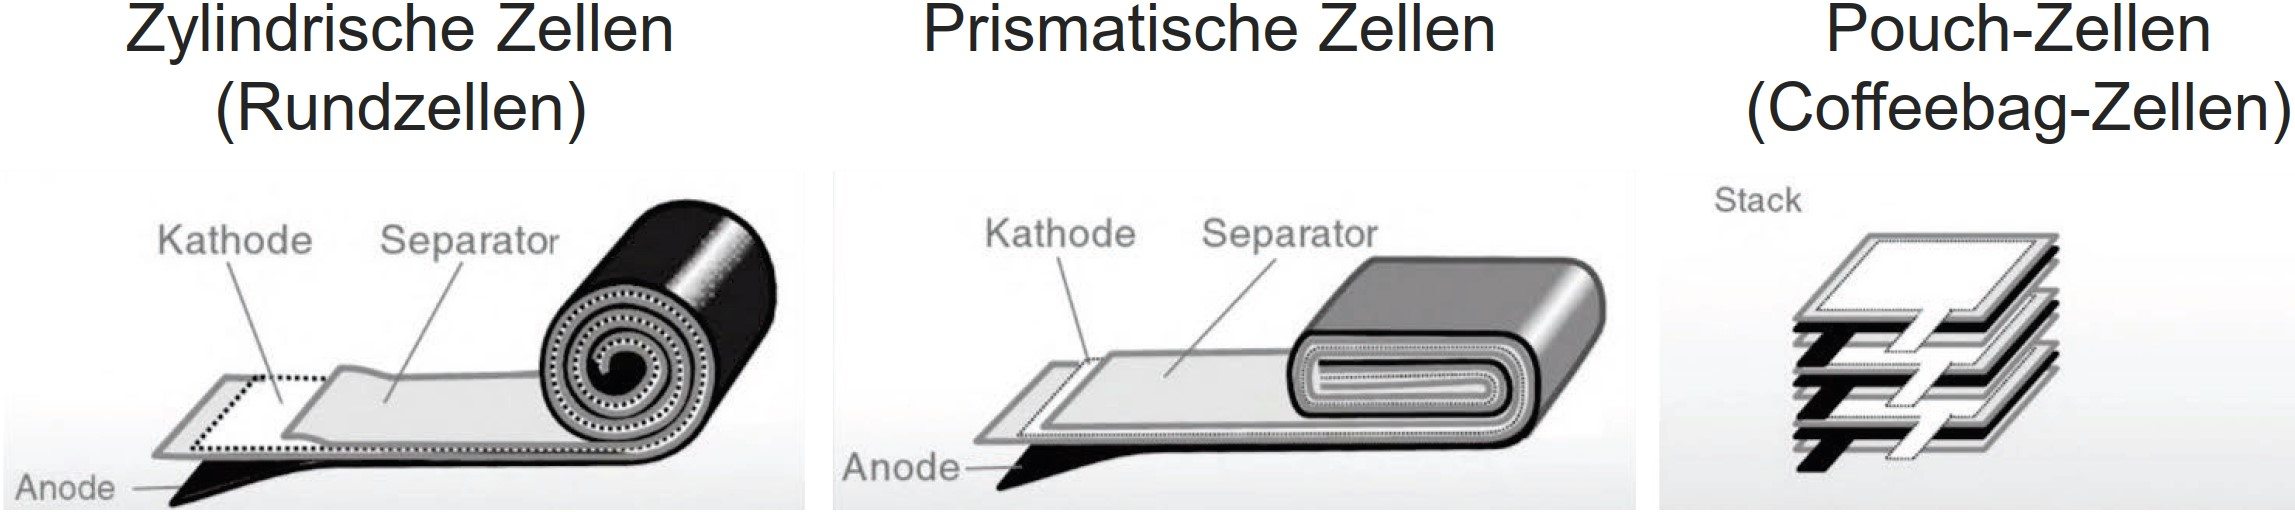
\includegraphics[width=0.98\columnwidth]{images/Aufbau_Batterie_1.jpg}


\columnbreak
\subsubsection{Ladeverfahren}

Typisch: I/U-Laden bzw. CCCV-Verfahren (Constant Current/Constant Voltage)\\
\begin{center}
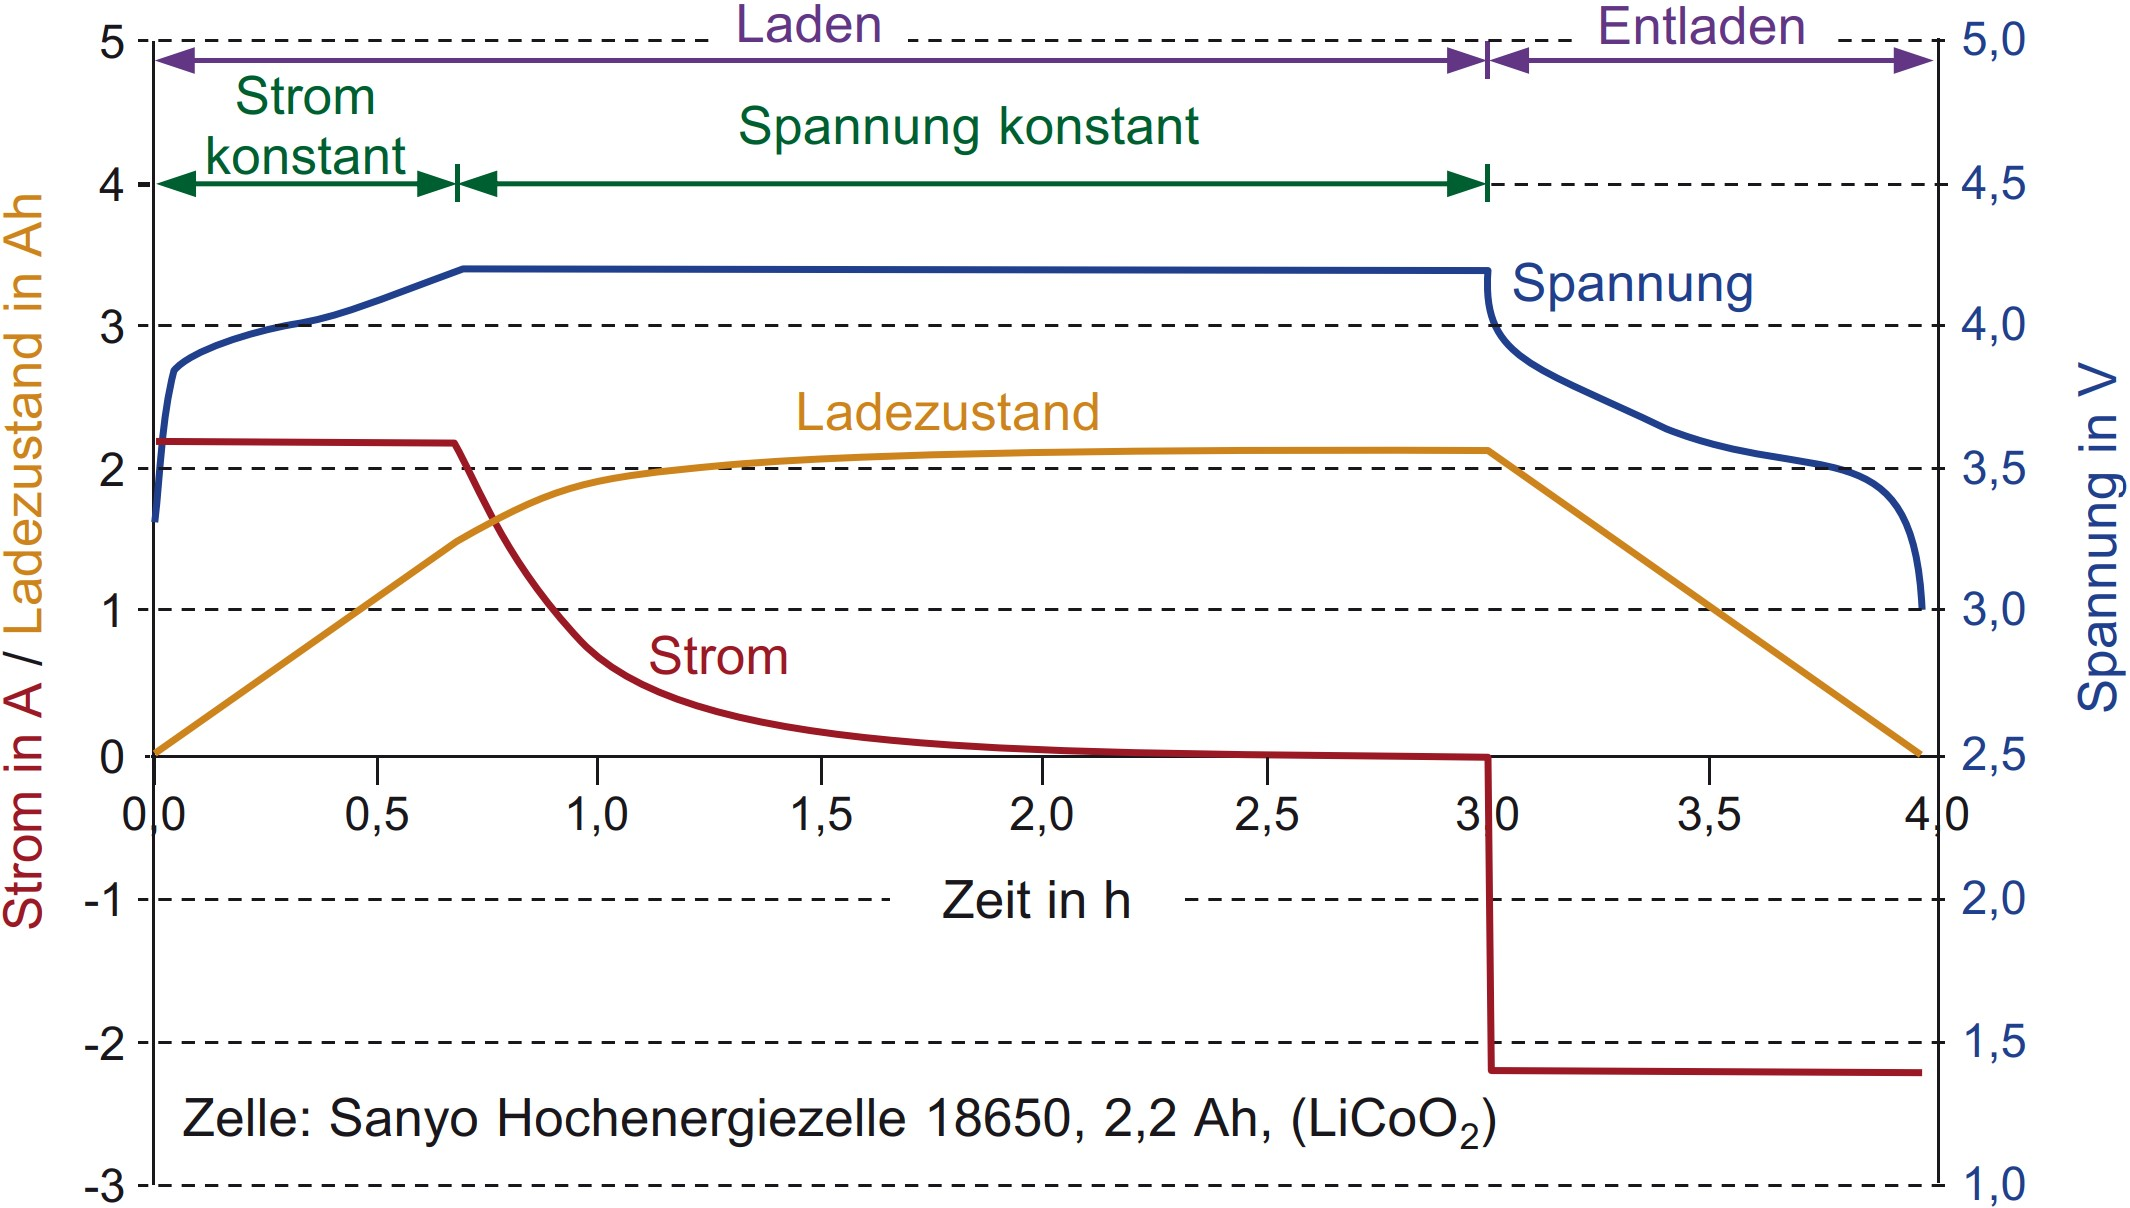
\includegraphics[width=0.8\columnwidth]{images/Lithium_Ionen_Akku.jpg}
\end{center}

Typisch ist eine Ladung nach dem CCCV-Verfahren (Constant Current / Constant Voltage) oder auch I/U-Ladung genannt. Dabei wird die Batterie zunächst mit einem konstanten Strom geladen. Sobald die Ladeschlussspannung erreicht ist, wird auf eine konstante Ladespannung umgeschaltet, um die Batterie vollständig aufzuladen aber nicht zu überladen.




\subsubsection{Kapazität}
Unter anderem abhängig von Entladestrom und Temperatur



\subsubsection{Alterung}


\begin{minipage}[t]{0.48\columnwidth}
\textbf{Kalendarische Alterung}
  \begin{itemize}
    \item Temperatur
    \item Ladezustand
  \end{itemize}
\end{minipage}
\hfill
\begin{minipage}[t]{0.48\columnwidth}
\textbf{Zyklenfestigkeit}
  \begin{itemize}
    \item Lade- und Entladerate
    \item Temperatur
    \item Ladezustand
    \item Entladetiefe
  \end{itemize}
\end{minipage}



\subsubsection{Vor- und Nachteile}

\begin{minipage}{0.48\textwidth}
\textbf{Vorteile}
\begin{itemize}
  \item Höchste Energiedichte und Wirkungsgrade
  \item Hohe Leistungsfähigkeit
  \item Keine spez. Standortanforderungen
  \item Schnellladefähigkeit
  \item Sehr geringe Selbstentladung (< 3\,\% pro Jahr bei Raumtemperatur, bis 15\,\% bei hohen Temperaturen)
  \item Grosses Anwendungsspektrum im stationären und mobilen Bereich
  \item Grosse Stückzahlen führen zu Kostensenkung
  \item Grösster Hoffnungsträger, höchste Forschungs- und Entwicklungstätigkeit
  \item Entwicklung neuer Aktivmaterialien
\end{itemize}
\end{minipage}
\hfill
\begin{minipage}{0.48\textwidth}
\textbf{Nachteile}
\begin{itemize}
  \item Keine inhärente Sicherheit (thermisches Durchgehen)
  \item Aufwändiges Batteriemanagementsystem für Sicherheit und Lebensdauer, Einzelzellüberwachung
  \item Lebensdauer begrenzt bei Ladezuständen ausserhalb 30--70\,\%
  \item Entnehmbare Kapazität sinkt bei tiefen Temperaturen
  \item Herstellung (Packaging) und Kühlung aufwendig
  \item (Noch) hohe Kosten
  \item Umweltverträglichkeit beim Lithiumabbau, soziale Akzeptanzprobleme
  \item Begrenzte Vorkommen an Lithium und weiteren Rohstoffen
\end{itemize}
\end{minipage}


\columnbreak
\subsection{Bleibatterie}
\subsubsection{Typen}

\begin{itemize}
  \item Pufferbetrieb (Autobatterie) vs. Zyklenbetrieb (Solarbatterie)

  \item Typische Solarbatterien
  \begin{itemize}
    \item Unterscheidung nach Elektrolyt
    \begin{itemize}
      \item \textbf{Blei-Säure-Batterie}
      \begin{itemize}
        \item Raumbelüftung (Gasung)
        \item Nachfüllen von Wasser
      \end{itemize}

      \item \textbf{Blei-Gel-Batterie}
      \begin{itemize}
        \item Elektrolyt durch Zusätze zu einem Gel verdickt $\rightarrow$ auslaufsicher
        \item Kein Gasaustritt $\rightarrow$ kein Nachfüllen von Wasser
        \item Wichtig: Einhaltung der Ladeschlussspannung (sonst Gasung)
      \end{itemize}
    \end{itemize}
    \item Unterscheidung nach Aufbau der Elektroden
        \begin{itemize}
        \item Blockbatterien (Blockakkus) mit mehreren Bleistäben von einer gemeinsamen Schutzhülle umgeben
        \item ortsfeste Panzerplattenbatterien, bei denen jeder Bleistab von einer Schutzhülle umgeben ist
      \end{itemize}
  \end{itemize}
\end{itemize}



\subsubsection{Vor- und Nachteile}

\begin{minipage}[t]{0.48\textwidth}
\textbf{Vorteile}
\begin{itemize}
  \item Etablierteste Batterietechnologie, weltweit lange Erfahrungen, seit 150 Jahren im Einsatz
  \item Relativ kostengünstiges Batteriesystem
  \item Akzeptable Energie- und Leistungsdichte für stationäre Anwendungen
  \item Hohe Sicherheit im Vergleich zu Lithium- oder Natrium-Batterien
  \item Kein komplexes Zellmanagement erforderlich
  \item Vollladung unschädlich
  \item Unabhängig von Standortbedingungen
  \item Vollautomatisierte Massenproduktion ermöglicht Kostensenkung
  \item Viele Hersteller weltweit
  \item Günstigster Speicher für Inselnetze
\end{itemize}
\end{minipage}
\hfill
\begin{minipage}[t]{0.48\textwidth}
\textbf{Nachteile}
\begin{itemize}
  \item Schädliche Tiefentladungen
  \item Lange Standzeiten mit tiefen Ladezuständen vermeiden
  \item Gutes Temperaturmanagement erforderlich
  \item Batterieraumbelüftung erforderlich (Blei-Säure)
  \item Lade- und Entladefähigkeit nicht symmetrisch
  \item Begrenzte Zyklenlebensdauer
  \item Konkurrenz durch Kostensenkung bei Lithium-Batterien
  \item Begrenzte Bleilagerstätten
  \item Umweltverträglichkeit
\end{itemize}
\end{minipage}

\vspace{0.1cm}

\textbf{Vorteile gegenüber Lithium-Ionen-Batterien}

\begin{enumerate}
    \item Bleibatterien haben eine hohe Sicherheit (kein thermisches Durchgehen), weshalb auch kein komplexes Zellmanagement notwendig ist. Sie können eher an entlegenen Standorten unbeaufsichtigt gelassen werden.
    \item Eine Vollladung ist unschädlich. In netzfernen Anwendungen wird häufig über eine längere Zeit kein Verbraucher betrieben, es soll aber nach Möglichkeit jederzeit die volle Batteriekapazität zur Verfügung stehen.
\end{enumerate}



\subsection{Nickel-Batterie}


  \textbf{Nickel-Batterien}
  \begin{itemize}
    \item Entwickelt für höhere Energiedichte und Robustheit als Blei
    \item Diverse Typen, in der praktischen Anwendung dominieren:
  \end{itemize}

  \textbf{Nickel-Cadmium (NiCd)}
  \begin{itemize}
    \item Cadmium giftig, daher sinkt die Verwendung, teils verboten
    \item \glqq Memory\grqq-Effekt
    \item Anwendung bei sicherheitskritischen Anwendungen
  \end{itemize}

  \textbf{Nickel-Metall-Hydrid (NiMH)}
  \begin{itemize}
    \item Für Anwendungen im Hochleistungsbereich entwickelt
    \item Etwa doppelte Energiedichte gegenüber NiCd, Leistungsdichte ebenfalls wesentlich höher
    \item Geringerer maximaler Lade- und Entladestrom, kleinerer Temperaturbereich als NiCd, empfindlich gegen Überladung, Überhitzung, falsche Polung, Tiefentladung
    \item Anwendung in Consumerelektronik und Hybridfahrzeugen
  \end{itemize}



\subsubsection{Vor- und Nachteile Nickel-Batterie}

\begin{minipage}{0.48\textwidth}
\textbf{Vorteile}
\begin{itemize}
  \item Einsatz bei tiefen Temperaturen und extremen Umgebungsbedingungen möglich
  \item Tolerant gegenüber Tiefentladung und unterschiedlichen Ladezuständen, können tiefentladen und in jedem Ladezustand gelagert werden
  \item Hohe zyklische und kalendarische Lebensdauer
  \item Hohe Energiedichte
  \item Einsatz im Hochleistungsbereich
\end{itemize}
\end{minipage}
\hfill
\begin{minipage}{0.48\textwidth}
\textbf{Nachteile}
\begin{itemize}
  \item Hohe Kosten für Nickel
  \item Konkurrenz durch Kostensenkung bei Lithium-Batterien
  \item Giftiges Cadmium (bei NiCd)
\end{itemize}
\end{minipage}


\columnbreak
\subsection{Natrium-Batterie}


\textbf{Natrium-Hochtemperatur-Batterien}
  \begin{itemize}
    \item Wärmeisolierter Behälter mit Heizung und Kühlung, BMS erforderlich
    \item Geringe elektrochemische Selbstentladung, aber hohe \glqq thermische Selbstentladung\grqq
  \end{itemize}

\textbf{Natrium-Schwefel-Batterien}
  \begin{itemize}
    \item Betriebstemperatur: 300--350\,\textdegree C
    \item Hohe Zyklenzahl, abhängig von Entladetiefe
    \item Tiefentladung schädlich, verkürzt Lebensdauer, wird i.\,d.\,R. durch BMS vermieden
    \item Hoher Wirkungsgrad, aber thermische Verluste durch Heizung
    \item Betriebssicherheit: Bei Unfällen können durch Reaktionen Temperaturen über 1'000\,\textdegree C entstehen
    \item Anwendung: Grössere stationäre Anwendungen, z.\,B. für Regelenergie
    \end{itemize}

\textbf{Natrium-Nickelchlorid-Batterie (Salzschmelzbatterie, Zebra-Batterie)}
  \begin{itemize}
    \item Betriebstemperatur: 250--350\,\textdegree C
    \item Umweltfreundlich, keine seltenen Materialien (Kochsalz, Nickel, Eisen, Keramik)
    \item Abgekühlt praktisch unbegrenzt lagerfähig, keine Selbstentladung
    \item Grosser Temperaturbereich: $-20$ bis $+60\,^\circ$C
    \item Anwendung: Mobilfunk-Basisstationen, mittelgrosse stationäre Anwendungen, Elektromobilität, Waffensysteme
  \end{itemize}

\textbf{Salzwasserbatterie (wässrige Natrium-Ionen-Batterie)}
  \begin{itemize}
    \item Niedertemperaturbatterie
    \item Geringe Spannung und dadurch niedrige Energiedichte (volumetrisch)
    \item Entnehmbare Kapazität stark abhängig von Entladestromstärke, daher C-Raten bis max. 0{,}25 empfohlen
    \item Anwendung: Heim- und Gewerbespeicher
  \end{itemize}



\subsubsection{Vor- und Nachteile Natrium-Batterie}

\begin{minipage}{0.48\textwidth}
\textbf{Vorteile}
\begin{itemize}
  \item Günstige Rohstoffe
  \item Wenig Einschränkung in Verfügbarkeit der Rohstoffe
  \item Sehr gute Umweltverträglichkeit
  \item Keine lokalen Voraussetzungen, kein Gefahrgut
  \item Hohe Zyklen-, lange kalendarische Lebensdauer
  \item Viele bestehende stationäre Anlagen
  \item Viele auslaufende Patente, neue Hersteller
  \item Hochtemperatur: Hohe Energiedichte
  \item Salzwasser-/Salzschmelze: nicht brennbar, nicht explosiv
  \item Salzwasser: tiefentladefest
\end{itemize}
\end{minipage}
\hfill
\begin{minipage}{0.48\textwidth}
\vspace{0.1cm}
\textbf{Nachteile}
\begin{itemize}
  \item Salzwasser: geringe Energiedichte und Entladeleistung
  \item Hochtemperatur-Batterien:
  \begin{itemize}
    \item Hoher Aufwand für Heizung und Kühlung
    \item Thermische Verluste
    \item Hohe Selbstentladung bei längeren Stillstandszeiten
    \item Gefahrenpotenzial aufgrund hoher Betriebstemperatur
  \end{itemize}
  \item NaS: Sicherheitsprobleme (Brand)
  \item Isolation von Natrium gegenüber Umwelteinflüssen (v.\,a. Wasser)
  \item Nur wenige Hersteller
  \item Konkurrenz zu Blei-Säure- und Li-Ion-Batterien
\end{itemize}
\end{minipage}



\subsection{Redox-Flow-Batterie}

\begin{itemize}
  \item Die Elektrolyte zirkulieren in zwei getrennten Kreisläufen, verbunden nur durch eine ionenleitende Membran
  \item Externer Speicher: unabhängige Dimensionierung von Leistung und Energie
  \begin{itemize}
    \item Schnelle \glqq Ladbarkeit\grqq{} durch Austausch der Elektrolyten
  \end{itemize}
  \item Betriebstemperatur: 20--30\,\textdegree C, über 40\,\textdegree C gefährlich
  \begin{itemize}
    \item BMS notwendig zur Steuerung von Temperatur, Spannung und Strom für optimalen Betriebspunkt
  \end{itemize}
  \item Wirkungsgrad der Zelle ca. 90\,\%, durch Peripheriegeräte (z.\,B. Pumpen) sinkt Systemwirkungsgrad auf 70--80\,\%
  \item Gute Vermeidbarkeit von Selbstentladung, da Elektrolytflüssigkeiten getrennt sind
  \item Anwendung:
  \begin{itemize}
    \item Große Speicherkapazitäten
    \item Lastspitzenausgleich und Spannungsstützung
    \item Bereitstellung von Regel- und Ausgleichsenergie
    \item Backup-/USV-Systeme zur Notstromversorgung
    \item Potenziell: Inselnetze, Elektromobilität
  \end{itemize}
\end{itemize}



\subsubsection{Vor- und Nachteile Redox-Flow-Batterie}

\begin{minipage}{0.48\textwidth}
\textbf{Vorteile}
\begin{itemize}
  \item Energie und Leistung unabhängig skalierbar
  \item Räumliche Trennung von Speicherbehälter und Reaktionszelle
  \item Hohe Zyklenlebensdauer, tiefentladefähig
  \item Lade- und Entladestrategien nicht so wichtig (im Vergleich zu Blei oder Lithium)
  \item Geringer Wartungsaufwand
  \item Einsatz unterschiedlicher Redoxpaare, neue Materialkombinationen, kein Ressourcenengpass
  \item Materialverbesserungen ermöglichen Wirkungsgradsteigerung und Kostensenkung; wirtschaftlich vorteilhaft bei hohem Verhältnis von Kapazität zu Leistung
  \item Viele auslaufende Patente, steigender Wettbewerbsdruck
  \item Standorte unbeschränkt
  \item Gute Umweltverträglichkeit
\end{itemize}
\end{minipage}
\hfill
\begin{minipage}{0.48\textwidth}
\textbf{Nachteile}
\begin{itemize}
  \item Geringe Energie- und Leistungsdichte
  \item Säurehaltige Flüssigkeiten verursachen Leckagen
  \item Teure Speichermedien
  \item Wartungsaufwand für Pumpen
  \item Stromverbrauch der Pumpen
  \item Rechtliche Probleme bei Genehmigung durch große Säuremengen
\end{itemize}
\end{minipage}





\subsection{Übersicht Batterien}

\begin{tabular}{|l|c|c|c|c|}
\hline
\textbf{Eigenschaft} & \textbf{Blei} & \textbf{Li-Ionen} & \textbf{Salzschm.} & \textbf{Salzwasser} \\
\hline
Lebensdauer [Jahre] & 5--15 & 10--20 & >15 & ca. 15 \\
\hline
Zyklenfest. [Zyklen] & 500--3'000 & 3'000--10'000 & 4'500 & >5'000 \\
\hline
Entladetiefe [\%] & 50--70 & 90--95 & ca. 85 & 70--100 \\
\hline
Energiedichte $[\frac{\mathrm{Wh}}{\mathrm{kg}}]$ & 30--40 & 200--250 & 100--120 & ca. 40 \\
\hline
Selbstentl. & 3--5 $\frac{\%}{\mathrm{Monat}}$ & 3--5 $\frac{\%}{\mathrm{Jahr}}$ & 20 $\frac{\%}{\mathrm{Tag}}$ \textcolor{green}{Stb} & Gering \\
\hline
Wirkungsgrad [\%] & 75--85 & 90--98 & 85--95 & 80--90 \\
\hline
Betriebstemp. [\textdegree C] & -10 bis 40 & -5 bis 40 & -20 bis 60 & -5 bis 50 \\
\hline
Max. C-Rate [C] & 0.3--0.5 & 1--3 & \textcolor{red}{(E) $\frac{1}{2}$}, \textcolor{blue}{(L) $\frac{1}{4}$} & 0.25 \\
\hline
(1) $[\frac{\mathrm{CHF}}{\mathrm{kWh}}]$ & 100--300 & 500--1'000 & 550--1'000 & 800--1'200 \\
\hline
(2) $[\frac{\mathrm{CHF}}{\mathrm{kWh}}]$ & 170--500 & 540--1'080 & 650--1'300 & 940--1'400 \\
\hline
\end{tabular}

\vspace{0.1cm}

\textcolor{green}{Stb = Standby}, \textcolor{red}{E = Entladen}, \textcolor{blue}{L = Laden}, Salzschm. = Salzschmelze

(1) = Kosten bezogen auf Nennkapazität $C_{\mathrm{nenn}}$

(2) = Kosten bezogen auf nutzbare Kapazität $C_{\mathrm{nutz}}$






















